\newcommand{\ContrLearnAccuracyTrends}{
	\begin{figure}[H]
		\centering
		\begin{subfigure}[b]{0.475\textwidth}
			\centering
			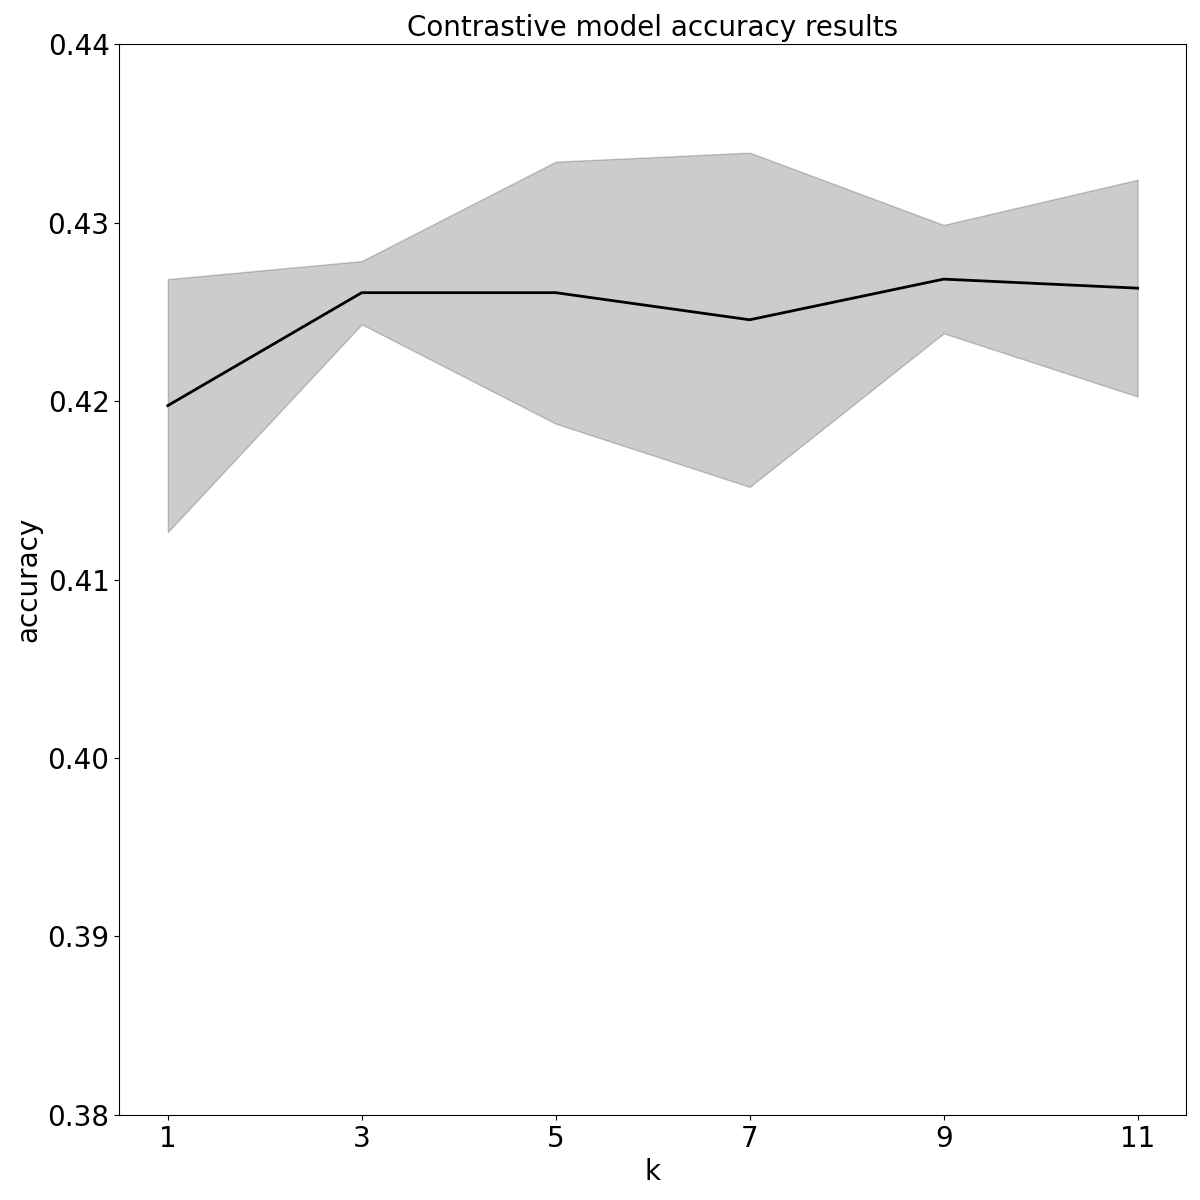
\includegraphics[width=\textwidth]{./results/joint_embedding_contr_learn_accuracy.png}
			\caption[]{{\small Contrastive \textbf{Joint Embedding}}}
			\label{fig:jointEmbeddingContrLearnAccuracyTrend}
		\end{subfigure}
		\hfill
		\begin{subfigure}[b]{0.475\textwidth}
			\centering
			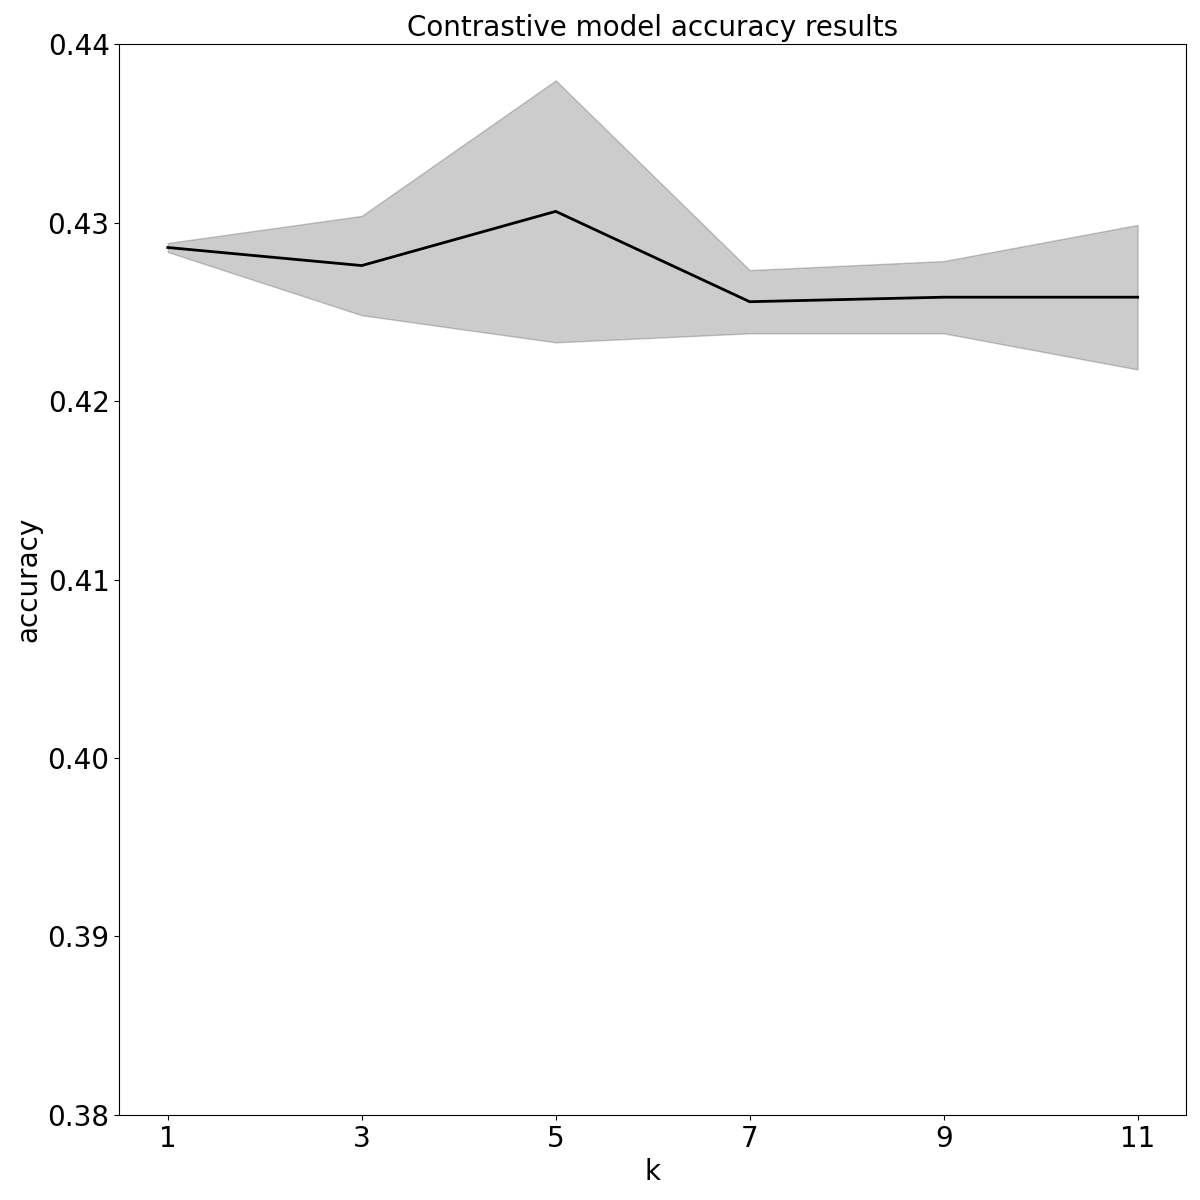
\includegraphics[width=\textwidth]{./results/mtje_contr_learn_accuracy.png}
			\caption[]{{\small Contrastive \textbf{MTJE} Model}}
			\label{fig:mtjeContrLearnAccuracyTrend}
		\end{subfigure}
		\vskip\baselineskip
		\begin{subfigure}[b]{0.475\textwidth}
			\centering
			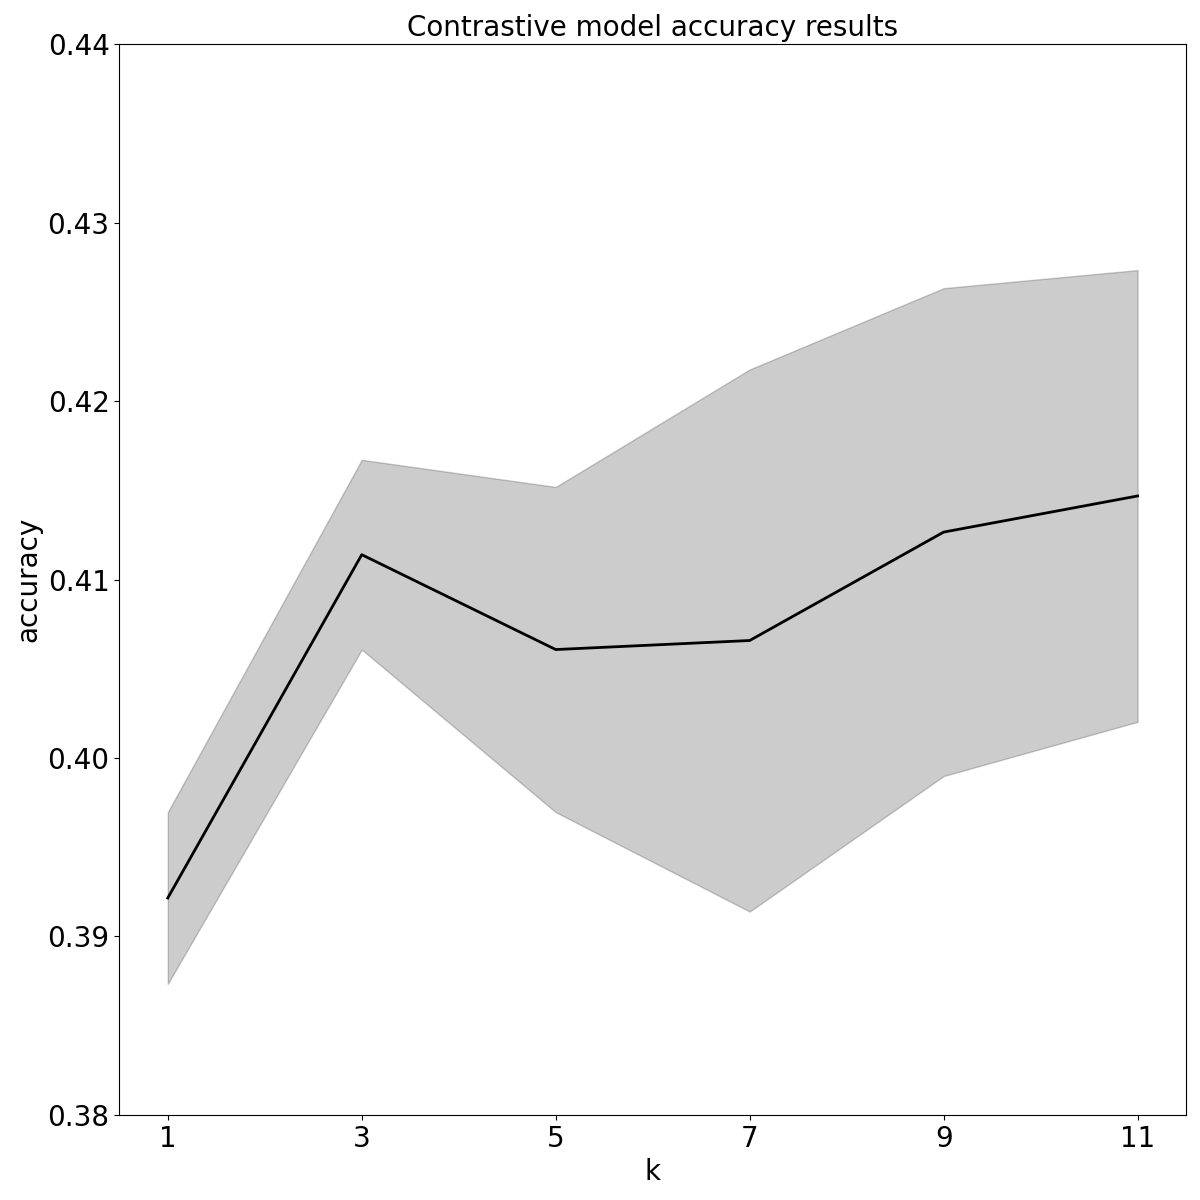
\includegraphics[width=\textwidth]{./results/contrastive_model_only_contr_learn_accuracy.png}
			\caption[]{{\small \textbf{Contrastive Model Only}}}
			\label{fig:ContrastiveModelOnlyContrLearnAccuracyTrend}
		\end{subfigure}
		\hfill
		\caption[Contrastive Model Accuracy Trends]{Mean and standard deviation of the accuracy trends obtained by evaluating the Contrastive Model based on the \textbf{Joint Embedding} and \textbf{MTJE} model implementations along with a Contrastive Model with no \textit{Transfer Learning} applied (\textbf{Contrastive Model Only}) on the malware family classification task using the k-NN algorithm as the number $k$ of nearest neighbours changes from 1 to 11. Results were aggregated over \textBF{3} training runs with different weight initializations and minibatch orderings.} \label{fig:ContrLearnAccuracyTrends}
	\end{figure}
}

\newcommand{\ContrLearnMrrAndMapResultsTable}{
	\begin{table}[H]
		\centering
		\begin{tabular}{|P{2cm}||P{3,2cm} P{3,2cm} P{3,2cm}|}
			\hline
			& Contrastive Joint Embedding & Contrastive MTJE Model & Contrastive Model Only \\
			\hline
			MRR & 0.506$\pm$0.008 & \textBF{0.509$\pm$0.002} & 0.503$\pm$0.011 \\
			MAP & 0.441$\pm$0.003 & \textBF{0.443$\pm$0.002} & 0.437$\pm$0.004 \\
			\hline
		\end{tabular}
		\caption[Contrastive Model family ranking MRR and MAP scores]{Mean and standard deviation MRR (Mean Reciprocal Rank) and MAP (Mean Average Precision) results obtained by evaluating the Contrastive Model based on the \textbf{Joint Embedding} and \textbf{MTJE} model implementations along with a Contrastive Model with no \textit{Transfer Learning} applied (\textbf{Contrastive Model Only}) on the Family Ranking task. Results were aggregated over \textBF{3} training runs with different weight initializations and minibatch orderings. Best results are shown in \textbf{bold}.} \label{tab:ContrLearnMrrAndMapResults}
	\end{table}
}

\newcommand{\ContrLearnAccuracyResultsTable}{
	\begin{table}[H]
		\centering
		\begin{tabular}{|P{2cm}||P{3,2cm} P{3,2cm} P{3,2cm}|}
			\hline
			& Contrastive Joint Embedding (with $k=9$) & Contrastive MTJE Model (with $k=5$) & Contrastive Model only (with $k=11$) \\
			\hline
			Accuracy & 0.427$\pm$0.003 & \textBF{0.431$\pm$0.007} & 0.415$\pm$0.013 \\
			\hline
		\end{tabular}
		\caption[Contrastive Model Accuracy Results]{Mean and Standard deviation of the accuracy obtained by evaluating the Contrastive Model based on the \textbf{Joint Embedding} and \textbf{MTJE} model along with a Contrastive Model with no \textit{Transfer Learning} applied (\textbf{Contrastive Model Only}) on the family classification task. Results were aggregated over \textBF{3} training runs with different weight initializations and minibatch orderings. Best results are shown in \textbf{bold}.} \label{tab:ContrLearnAccuracyResults}
	\end{table}
}

\newcommand{\ContrLearnScoresTable}{
	\begin{table}[H]
		\centering
		\begin{tabular}{|P{1,8cm}|P{1,3cm}||P{3cm} P{3cm} P{3cm}|}
			\hline
			& & Contrastive Joint Embedding (with $k=9$) & Contrastive MTJE Model (with $k=5$) & Contrastive Model only (with $k=11$) \\
			\hline
			\multirow{3}{4em}{Jaccard Similarity} & Micro & 0.271$\pm$0.002 & \textBF{0.274$\pm$0.006} & 0.262$\pm$0.010 \\
			& Macro & 0.310$\pm$0.006 & \textBF{0.313$\pm$0.003} & 0.292$\pm$0.008 \\
			& Weighted & 0.310$\pm$0.007 & \textBF{0.314$\pm$0.003} & 0.291$\pm$0.009 \\
			\hline
			\multirow{3}{4em}{Recall} & Micro & 0.427$\pm$0.003 & \textBF{0.431$\pm$0.007} & 0.415$\pm$0.013 \\
			& Macro & 0.427$\pm$0.002 & \textBF{0.430$\pm$0.007} & 0.415$\pm$0.012 \\
			& Weighted & 0.427$\pm$0.003 & \textBF{0.431$\pm$0.007} & 0.415$\pm$0.013 \\
			\hline
			\multirow{3}{4em}{Precision} & Micro & 0.427$\pm$0.003 & \textBF{0.431$\pm$0.007} & 0.415$\pm$0.013 \\
			& Macro & 0.481$\pm$0.003 & \textBF{0.502$\pm$0.008} & 0.469$\pm$0.014 \\
			& Weighted & 0.481$\pm$0.004 & \textBF{0.501$\pm$0.009} & 0.469$\pm$0.014 \\
			\hline
			\multirow{3}{4em}{F1-score} & Micro & 0.427$\pm$0.003 & \textBF{0.431$\pm$0.007} & 0.415$\pm$0.013 \\
			& Macro & 0.433$\pm$0.006 & \textBF{0.434$\pm$0.001} & 0.400$\pm$0.003 \\
			& Weighted & 0.433$\pm$0.007 & \textBF{0.435$\pm$0.001} & 0.400$\pm$0.004 \\
			\hline
		\end{tabular}
		\caption[Contrastive Model Scores]{Mean and Standard deviation of the multi-class classification scores obtained by evaluating the 2 Contrastive Models obtained by transferring the knowledge from a previous training run on the Sorel-20m dataset of the \textbf{Joint Embedding} and \textbf{MTJE} model implementations, respectively, along with a Contrastive Model with no \textit{Transfer Learning} applied (\textbf{Contrastive Model Only}) on the family classification task using the k-NN algorithm. Results were aggregated over \textBF{3} training runs with different weight initializations and minibatch orderings. Best results are shown in \textbf{bold}.} \label{tab:ContrLearnScoresTable}
	\end{table}
}

\newcommand{\ContrLearnJointEmbeddingConfusionMatrix}{
	\begin{figure}[H]
		\vspace*{-0.5cm}
		\centering
		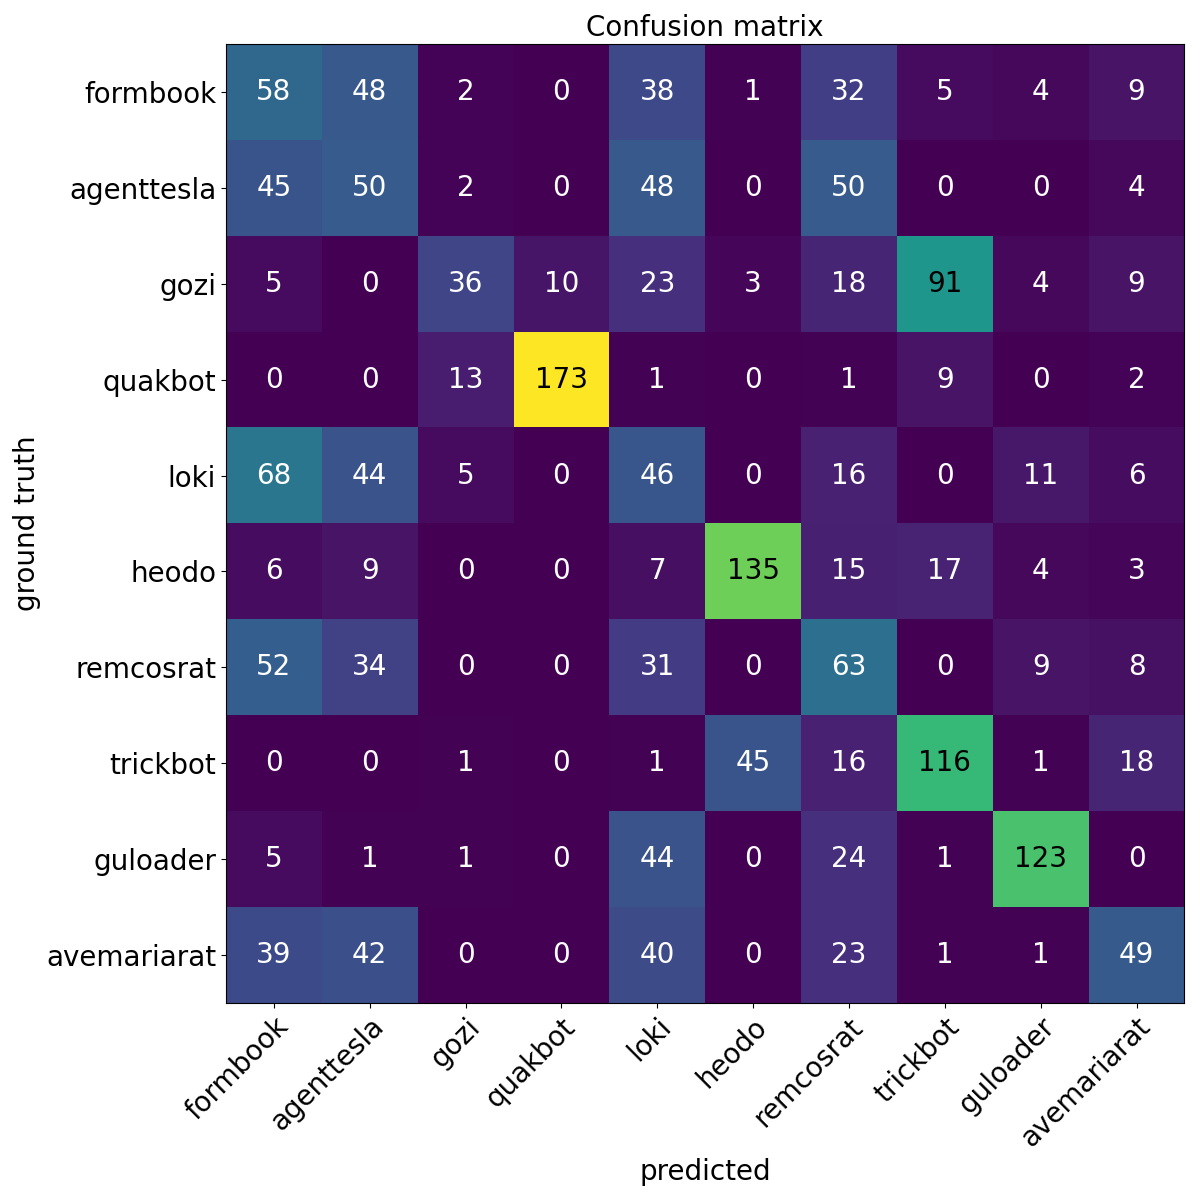
\includegraphics[width=0.7\textwidth]{./results/joint_embedding_contr_learn_9-nn_confusion_matrix.png}
		\vspace*{-0.2cm}
		\caption[Contrastive Model based on Joint Embedding Confusion Matrix]{Confusion Matrix resulting from the evaluation of the Contrastive Model obtained by transferring the knowledge from a previous \textbf{Joint Embedding} model training run on the Sorel-20m dataset on the family classification task using the k-NN algorithm with $k=9$.}
		\label{fig:ContrLearnJointEmbeddingConfusionMatrix}
		\vspace*{-0.2cm}
	\end{figure}
}

\newcommand{\ContrLearnMtjeConfusionMatrix}{
	\begin{figure}[H]
		\vspace*{-0.5cm}
		\centering
		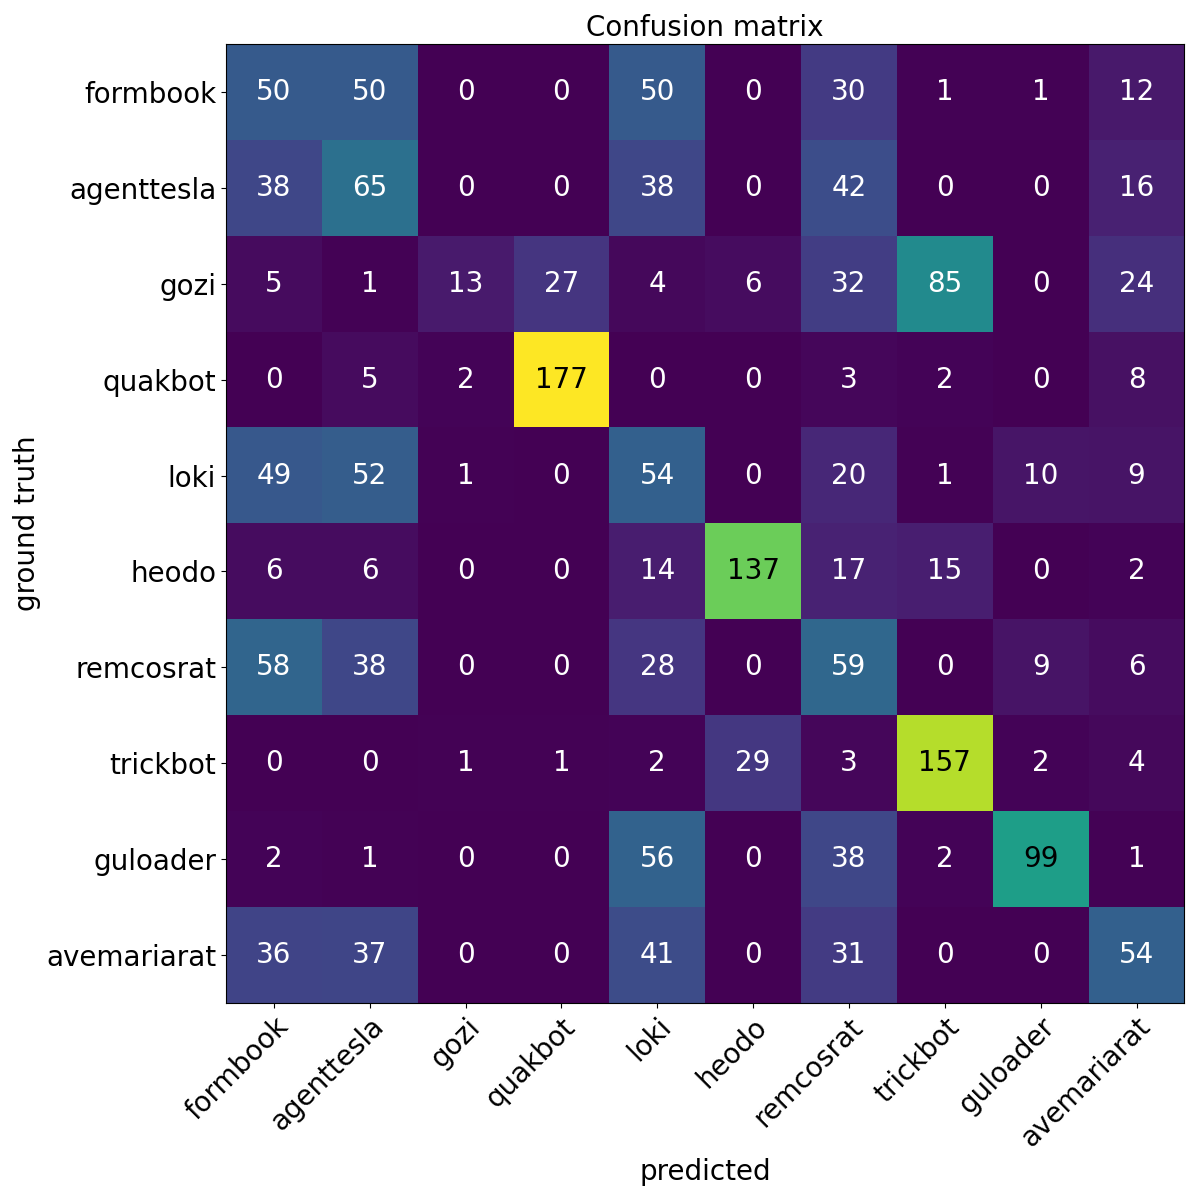
\includegraphics[width=0.7\textwidth]{./results/mtje_contr_learn_5-nn_confusion_matrix.png}
		\vspace*{-0.2cm}
		\caption[Contrastive Model based on MTJE Model Confusion Matrix]{Confusion Matrix resulting from the evaluation of the Contrastive Model obtained by transferring the knowledge from a previous \textbf{MTJE} model training run on the Sorel-20m dataset on the family classification task using the k-NN algorithm with $k=5$.}
		\label{fig:ContrLearnMtjeConfusionMatrix}
		\vspace*{-0.2cm}
	\end{figure}
}

\newcommand{\ContrLearnOnlyConfusionMatrix}{
	\begin{figure}[H]
		\vspace*{-0.5cm}
		\centering
		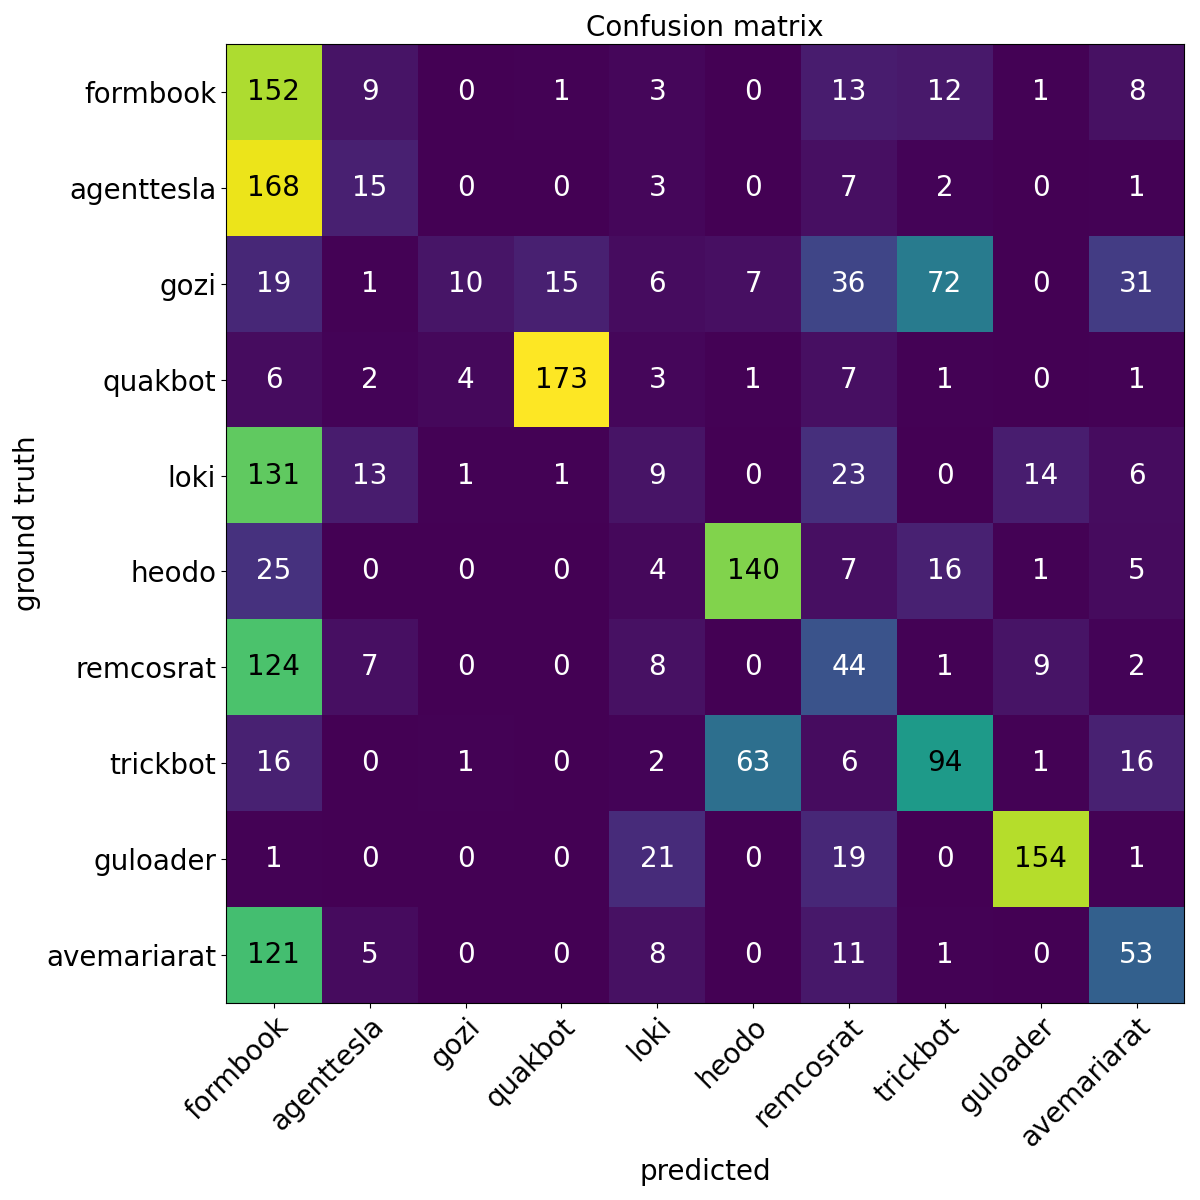
\includegraphics[width=0.7\textwidth]{./results/contrastive_model_only_contr_learn_11-nn_confusion_matrix.png}
		\vspace*{-0.2cm}
		\caption[Contrastive Model Only Joint Embedding Confusion Matrix]{Confusion Matrix resulting from the evaluation of the Contrastive Model trained from scratch (with no transfer learning) on the family classification task using the k-NN algorithm with $k=11$.}
		\label{fig:ContrLearnOnlyConfusionMatrix}
		\vspace*{-0.2cm}
	\end{figure}
}

\newcommand{\ContrLearnMaxApExampleRankTable}{
	\begin{table}[H]
		\centering
		\begin{tabular}{|P{1,4cm}||P{1,1cm} P{0,4cm} P{1,5cm}|P{1,1cm} P{0,4cm} P{1,5cm}|P{1,1cm} P{0,4cm} P{1,5cm}|}
			\hline
			Max AP & \multicolumn{3}{c|}{Contrastive} & \multicolumn{3}{c|}{Contrastive} & \multicolumn{3}{c|}{Contrastive} \\
			& \multicolumn{3}{c|}{Joint Embedding} & \multicolumn{3}{c|}{MTJE Model} & \multicolumn{3}{c|}{Model Only} \\
			& Sha256 & Label & Family & Sha256 & Label & Family & Sha256 & Label & Family \\
			\hline
			Query & 2d2796.. & 8 & guloader & 35287c.. & 8 & guloader & 15c19c.. & 5 & heodo \\
			\hline
			0 & \textBF{2bb8df}.. & \textBF{8} & \textBF{guloader} & \textBF{22b138}.. & \textBF{8} & \textBF{guloader} & \textBF{4a36c2}.. & \textBF{5} & \textBF{heodo} \\
			1 & \textBF{62b561}.. & \textBF{8} & \textBF{guloader} & \textBF{5f9b8c}.. & \textBF{8} & \textBF{guloader} & \textBF{bbcda6}.. & \textBF{5} & \textBF{heodo} \\
			2 & \textBF{3b6bd5}.. & \textBF{8} & \textBF{guloader} & \textBF{ea8a5f}.. & \textBF{8} & \textBF{guloader} & \textBF{445915}.. & \textBF{5} & \textBF{heodo} \\
			3 & \textBF{279013}.. & \textBF{8} & \textBF{guloader} & \textBF{34cc64}.. & \textBF{8} & \textBF{guloader} & \textBF{cafc08}.. & \textBF{5} & \textBF{heodo} \\
			4 & \textBF{2d2e4e}.. & \textBF{8} & \textBF{guloader} & \textBF{024efd}.. & \textBF{8} & \textBF{guloader} & \textBF{912186}.. & \textBF{5} & \textBF{heodo} \\
			5 & \textBF{7174dc}.. & \textBF{8} & \textBF{guloader} & \textBF{ac74bf}.. & \textBF{8} & \textBF{guloader} & \textBF{f906c1}.. & \textBF{5} & \textBF{heodo} \\
			6 & \textBF{092150}.. & \textBF{8} & \textBF{guloader} & \textBF{f12049}.. & \textBF{8} & \textBF{guloader} & \textBF{9662b2}.. & \textBF{5} & \textBF{heodo} \\
			7 & \textBF{69d83c}.. & \textBF{8} & \textBF{guloader} & \textBF{28d54a}.. & \textBF{8} & \textBF{guloader} & \textBF{34a0a3}.. & \textBF{5} & \textBF{heodo} \\
			8 & \textBF{314e93}.. & \textBF{8} & \textBF{guloader} & \textBF{a28301}.. & \textBF{8} & \textBF{guloader} & \textBF{63f16a}.. & \textBF{5} & \textBF{heodo} \\
			9 & \textBF{2a44e9}.. & \textBF{8} & \textBF{guloader} & \textBF{ab58ae}.. & \textBF{8} & \textBF{guloader} & \textBF{30b629}.. & \textBF{5} & \textBF{heodo} \\
			\hline
			Max AP & \multicolumn{3}{c|}{1.000} & \multicolumn{3}{c|}{1.000} & \multicolumn{3}{c|}{1.000} \\
			\hline
		\end{tabular}
		\vspace{-0.2cm}
		\caption[Contrastive Model family ranking max AP example]{Example rankings (limited to the first 10 samples) having the maximum Average Precision (\textbf{max AP}) between the ones produced by the 2 Contrastive Models obtained by transferring the knowledge from a previous training run of the \textbf{Joint Embedding} and \textbf{MTJE} model implementations, respectively, and by a Contrastive Model with no \textit{Transfer Learning} applied (\textbf{Contrastive Model Only}). The elements matching the query sample are shown in \textbf{bold}.} \label{tab:ContrLearnMaxApExampleRank}
		\vspace{-0.2cm}
	\end{table}
}

\newcommand{\ContrLearnMaxRrExampleRankTable}{
	\begin{table}[H]
		\centering
		\begin{tabular}{|P{1,4cm}||P{1,1cm} P{0,4cm} P{1,5cm}|P{1,1cm} P{0,4cm} P{1,5cm}|P{1,1cm} P{0,4cm} P{1,5cm}|}
			\hline
			Max RR & \multicolumn{3}{c|}{Contrastive} & \multicolumn{3}{c|}{Contrastive} & \multicolumn{3}{c|}{Contrastive} \\
			& \multicolumn{3}{c|}{Joint Embedding} & \multicolumn{3}{c|}{MTJE Model} & \multicolumn{3}{c|}{Model Only} \\
			& Sha256 & Label & Family & Sha256 & Label & Family & Sha256 & Label & Family \\
			\hline
			Query & 7308f0.. & 3 & quakbot & 35287c.. & 8 & guloader & 9e955c.. & 7 & trickbot \\
			\hline
			0 & \textBF{770919}.. & \textBF{3} & \textBF{quakbot} & \textBF{22b138}.. & \textBF{8} & \textBF{guloader} & \textBF{973029}.. & \textBF{7} & \textBF{trickbot} \\
			1 & \textBF{27dd2f}.. & \textBF{3} & \textBF{quakbot} & \textBF{5f9b8c}.. & \textBF{8} & \textBF{guloader} & 4c3ccb.. & 5 & heodo \\
			2 & \textBF{dfae1e}.. & \textBF{3} & \textBF{quakbot} & \textBF{ea8a5f}.. & \textBF{8} & \textBF{guloader} & \textBF{d0de78}.. & \textBF{7} & \textBF{trickbot} \\
			3 & \textBF{246a1e}.. & \textBF{3} & \textBF{quakbot} & \textBF{34cc64}.. & \textBF{8} & \textBF{guloader} & \textBF{537cae}.. & \textBF{7} & \textBF{trickbot} \\
			4 & \textBF{6c0091}.. & \textBF{3} & \textBF{quakbot} & \textBF{024efd}.. & \textBF{8} & \textBF{guloader} & \textBF{a0e0ca}.. & \textBF{7} & \textBF{trickbot} \\
			5 & \textBF{184a00}.. & \textBF{3} & \textBF{quakbot} & \textBF{ac74bf}.. & \textBF{8} & \textBF{guloader} & \textBF{27311e}.. & \textBF{7} & \textBF{trickbot} \\
			6 & \textBF{d15b9a}.. & \textBF{3} & \textBF{quakbot} & \textBF{f12049}.. & \textBF{8} & \textBF{guloader} & \textBF{713ea2}.. & \textBF{7} & \textBF{trickbot} \\
			7 & \textBF{e64497}.. & \textBF{3} & \textBF{quakbot} & \textBF{28d54a}.. & \textBF{8} & \textBF{guloader} & \textBF{6ae0b4}.. & \textBF{7} & \textBF{trickbot} \\
			8 & \textBF{a66698}.. & \textBF{3} & \textBF{quakbot} & \textBF{a28301}.. & \textBF{8} & \textBF{guloader} & \textBF{128857}.. & \textBF{7} & \textBF{trickbot} \\
			9 & \textBF{8048dc}.. & \textBF{3} & \textBF{quakbot} & \textBF{ab58ae}.. & \textBF{8} & \textBF{guloader} & \textBF{02f92c}.. & \textBF{7} & \textBF{trickbot} \\
			\hline
			Max RR & \multicolumn{3}{c|}{1.000} & \multicolumn{3}{c|}{1.000} & \multicolumn{3}{c|}{1.000} \\
			\hline
		\end{tabular}
		\vspace{-0.2cm}
		\caption[Contrastive Model family ranking max RR example]{Example rankings (limited to the first 10 samples) having the maximum Reciprocal Rank (\textbf{max RR}) between the ones produced by the 2 Contrastive Models obtained by transferring the knowledge from a previous training run of the \textbf{Joint Embedding} and \textbf{MTJE} model implementations, respectively, and by a Contrastive Model with no \textit{Transfer Learning} applied (\textbf{Contrastive Model Only}). The elements matching the query sample are shown in \textbf{bold}.} \label{tab:ContrLearnMaxRrExampleRank}
		\vspace{-0.2cm}
	\end{table}
}

\newcommand{\ContrLearnMinApExampleRankTable}{
	\begin{table}[H]
		\centering
		\begin{tabular}{|P{1,4cm}||P{1,1cm} P{0,4cm} P{1,5cm}|P{1,1cm} P{0,4cm} P{1,5cm}|P{1,1cm} P{0,4cm} P{1,5cm}|}
			\hline
			Min AP & \multicolumn{3}{c|}{Contrastive} & \multicolumn{3}{c|}{Contrastive} & \multicolumn{3}{c|}{Contrastive} \\
			& \multicolumn{3}{c|}{Joint Embedding} & \multicolumn{3}{c|}{MTJE Model} & \multicolumn{3}{c|}{Model Only} \\
			& Sha256 & Label & Family & Sha256 & Label & Family & Sha256 & Label & Family \\
			\hline
			Query & a3b2db.. & 0 & formbook & 241991.. & 7 & trickbot & ff69d2.. & 2 & gozi \\
			\hline
			0 & adf26e.. & 7 & trickbot & 0417c3.. & 5 & heodo & a8bfae.. & 5 & heodo \\
			1 & 5271ab.. & 7 & trickbot & ecdeac.. & 5 & heodo & e0dda0.. & 5 & heodo \\
			2 & 623b7d.. & 7 & trickbot & c5a06a.. & 5 & heodo & e28d1b.. & 5 & heodo \\
			3 & 7db413.. & 7 & trickbot & 0f6356.. & 5 & heodo & 417fd8.. & 5 & heodo \\
			4 & 1689b8.. & 7 & trickbot & a9471c.. & 5 & heodo & 6ed52c.. & 5 & heodo \\
			5 & b544cd.. & 7 & trickbot & d9fc0b.. & 5 & heodo & f196bb.. & 5 & heodo \\
			6 & ea6a9b.. & 7 & trickbot & 5d000f.. & 5 & heodo & 596c44.. & 5 & heodo \\
			7 & 31652f.. & 7 & trickbot & 05509e.. & 5 & heodo & f249cd.. & 5 & heodo \\
			8 & 99f7ef.. & 7 & trickbot & 348634.. & 5 & heodo & b5105e.. & 5 & heodo \\
			9 & 2c9404.. & 7 & trickbot & d185f7.. & 5 & heodo & 7eba4d.. & 5 & heodo \\
			\hline
			Min AP & \multicolumn{3}{c|}{0.000} & \multicolumn{3}{c|}{0.000} & \multicolumn{3}{c|}{0.000} \\
			\hline
		\end{tabular}
		\vspace{-0.2cm}
		\caption[Contrastive Model family ranking max AP example]{Example rankings (limited to the first 10 samples) having the minimum Average Precision (\textbf{min AP}) between the ones produced by the 2 Contrastive Models obtained by transferring the knowledge from a previous training run of the \textbf{Joint Embedding} and \textbf{MTJE} model implementations, respectively, and by a Contrastive Model with no \textit{Transfer Learning} applied (\textbf{Contrastive Model Only}). The elements matching the query sample are shown in \textbf{bold}.} \label{tab:ContrLearnMinApExampleRank}
		\vspace{-0.2cm}
	\end{table}
}

\newcommand{\ContrLearnMinRrExampleRankTable}{
	\begin{table}[H]
		\centering
		\begin{tabular}{|P{1,4cm}||P{1,1cm} P{0,4cm} P{1,5cm}|P{1,1cm} P{0,4cm} P{1,5cm}|P{1,1cm} P{0,4cm} P{1,5cm}|}
			\hline
			Min RR & \multicolumn{3}{c|}{Contrastive} & \multicolumn{3}{c|}{Contrastive} & \multicolumn{3}{c|}{Contrastive} \\
			& \multicolumn{3}{c|}{Joint Embedding} & \multicolumn{3}{c|}{MTJE Model} & \multicolumn{3}{c|}{Model Only} \\
			& Sha256 & Label & Family & Sha256 & Label & Family & Sha256 & Label & Family \\
			\hline
			Query & a3b2db.. & 0 & formbook & 241991.. & 7 & trickbot & ff69d2.. & 2 & gozi \\
			\hline
			0 & adf26e.. & 7 & trickbot & 0417c3.. & 5 & heodo & a8bfae.. & 5 & heodo \\
			1 & 5271ab.. & 7 & trickbot & ecdeac.. & 5 & heodo & e0dda0.. & 5 & heodo \\
			2 & 623b7d.. & 7 & trickbot & c5a06a.. & 5 & heodo & e28d1b.. & 5 & heodo \\
			3 & 7db413.. & 7 & trickbot & 0f6356.. & 5 & heodo & 417fd8.. & 5 & heodo \\
			4 & 1689b8.. & 7 & trickbot & a9471c.. & 5 & heodo & 6ed52c.. & 5 & heodo \\
			5 & b544cd.. & 7 & trickbot & d9fc0b.. & 5 & heodo & f196bb.. & 5 & heodo \\
			6 & ea6a9b.. & 7 & trickbot & 5d000f.. & 5 & heodo & 596c44.. & 5 & heodo \\
			7 & 31652f.. & 7 & trickbot & 05509e.. & 5 & heodo & f249cd.. & 5 & heodo \\
			8 & 99f7ef.. & 7 & trickbot & 348634.. & 5 & heodo & b5105e.. & 5 & heodo \\
			9 & 2c9404.. & 7 & trickbot & d185f7.. & 5 & heodo & 7eba4d.. & 5 & heodo \\
			\hline
			Min RR & \multicolumn{3}{c|}{0.000} & \multicolumn{3}{c|}{0.000} & \multicolumn{3}{c|}{0.000} \\
			\hline
		\end{tabular}
		\vspace{-0.2cm}
		\caption[Contrastive Model family ranking max AP example]{Example rankings (limited to the first 10 samples) having the minimum Reciprocal Rank (\textbf{min RR}) between the ones produced by the 2 Contrastive Models obtained by transferring the knowledge from a previous training run of the \textbf{Joint Embedding} and \textbf{MTJE} model implementations, respectively, and by a Contrastive Model with no \textit{Transfer Learning} applied (\textbf{Contrastive Model Only}). The elements matching the query sample are shown in \textbf{bold}.} \label{tab:ContrLearnMinRrExampleRank}
		\vspace{-0.2cm}
	\end{table}
}